\section{Рабочий проект}
\subsection{Классы, используемые при разработке сайта}

Список классов и методов, которые были использованы при создании приложения представлены далее.

\renewcommand{\arraystretch}{0.8}

\subsubsection{Класс ANFIS}

Класс ANFIS относится к модулю нейронной сети и используется для идентификации объектов с помощью нечеткой нейросети.

Описание методов класса ANFIS представлено в таблице \ref{table:anfis_methods}.

\begin{xltabular}{\textwidth}{|X|X|}
\caption{Методы класса ANFIS}\label{table:anfis_methods} \\
\hline \centrow
Название метода & \centrow  Описание метода \\
\hline \centrow 1 & \centrow 2 \\ \hline
\endfirsthead
\caption*{Продолжение таблицы \ref{table:anfis_methods}}\\
\hline \centrow 1 & \centrow 2 \\ \hline
\finishhead
нормализацияКаналов(ПутьФайла) & Загрузка изображения из файла, разделение на цветовые каналы и преобразование в массивы с последующей нормализацией значений яркости. \\
\hline
АнфисаРаспознать(Путь, ИмяМодели) & Прием данных, обработанных методом нормализацияКаналов, и их обработка с использованием оптимизированной модели искусственной нейронной сети в модуле anfisReady. \\
\hline
АнфисаТренировать(Набор, Размер, ИмяМодели) & Инициация процесса обучения с использованием предоставленного набора данных для конфигурации и оптимизации модели нечеткой нейронной сети. \\
\hline
AnfisReady(data, name) & Передача данных в нейронную сеть на пиксельном уровне и вычисление степени соответствия каждого пикселя выбранной модели. \\
\hline
Anfis(data, name) & Процесс обучения нечеткой нейронной сети с использованием тренировочной выборки. \\
\hline
\end{xltabular}

\subsubsection{Класс DB}

Класс DB предназначен для работы с базой данных.

Описание методов класса DB представлено в таблице \ref{table:db_methods}.

\begin{xltabular}{\textwidth}{|X|X|}
\caption{Методы класса ANFIS}\label{table:db_methods} \\
\hline \centrow
Название метода & \centrow  Описание метода \\
\hline \centrow 1 & \centrow 2 \\ \hline
\endfirsthead
\caption*{Продолжение таблицы \ref{table:db_methods}}\\
\hline \centrow 1 & \centrow 2 \\ \hline
\finishhead
сохранить(ИмяМодели, Набор) & Архивация тренировочного датасета и обученной нейросетевой модели в базе данных. \\
\hline
загрузитьСписокНаборов() & Чтение и формирование списка доступных тренировочных наборов данных и моделей. \\
\hline
загрузитьНабор(Название) & Извлечение специфического обучающего набора из базы данных. \\
\hline
\end{xltabular}

\subsubsection{Класс main}

Класс main является частью графического интерфейса и обеспечивает взаимодействие с пользователем.

Описание методов класса main представлено в таблице \ref{table:main_methods}.

\begin{xltabular}{\textwidth}{|X|X|}
\caption{Методы класса ANFIS}\label{table:main_methods} \\
\hline \centrow
Название метода & \centrow  Описание метода \\
\hline \centrow 1 & \centrow 2 \\ \hline
\endfirsthead
\caption*{Продолжение таблицы \ref{table:main_methods}}\\
\hline \centrow 1 & \centrow 2 \\ \hline
\finishhead
загрузитьИзображение() & Загрузка и масштабирование изображения для отображения в пользовательском интерфейсе. \\
\hline
распознать() & Инициация процесса передачи изображения в нейронную сеть и выбора предварительно обученной модели. \\
\hline
выбрать(ОкноВыбора) & Интеграция модели в нейронную сеть и деактивация интерфейса выбора. \\
\hline
сохранитьРезультатРаспознания() & Активация интерфейса для сохранения результатов нейронной сети. \\
\hline
обучать() & Активация интерфейса для выбора набора данных для обучения сети. \\
\hline
подтвердить(ОкноВыбора) & Передача датасета для обучения и активация интерфейса для присвоения имени модели. \\
\hline
отправить(ОкноНазвания) & Трансмиссия наименования модели в нейронную сеть и инициация обучения. \\
\hline
\end{xltabular}
\renewcommand{\arraystretch}{1.0}

\subsection{Модульное тестирование разработанного приложения}

Модульные тесты для класса ANFIS из модели данных представлены на рисунках \ref{test1:image}-\ref{test3:image}.

\begin{figure}[H]
\begin{lstlisting}[language=Python]
import os
import unittest
from PIL import Image
import anfis
import numpy as np
import matlab
from random import shuffle
from ANFIS import нормализацияКаналов
from ANFIS import АнфисаРаспознать

class TestНормализацияКаналов(unittest.TestCase):
    def test_нормализация_существующего_файла(self):
        результат = нормализацияКаналов('test_image.png')
        self.assertIsNotNone(результат, "Функция должна возвращать не None для существующего файла")
        self.assertTrue((результат >= 0).all() and (результат <= 1).all(), "Все значения должны быть в диапазоне от 0 до 1")
    def test_нормализация_несуществующего_файла(self):
        результат = нормализацияКаналов('несуществующий_файл.jpg')
        self.assertIsNone(результат, "Функция должна возвращать None для несуществующего файла")
\end{lstlisting}  
\caption{Модульный тест метода нормализацияКаналов класса ANFIS}
\label{test1:image}
\end{figure}

\begin{figure}[H]
\begin{lstlisting}[language=Python]
import os
import unittest
from PIL import Image
import anfis
import numpy as np
import matlab
from random import shuffle
from ANFIS import нормализацияКаналов
from ANFIS import АнфисаРаспознать

class TestАнфисаРаспознать(unittest.TestCase):
    def setUp(self):
        self.путь = 'test_image.png'
        self.имяМодели = 'test_model_name'
    def test_распознавание_изображения(self):
        результат = АнфисаРаспознать(self.путь, self.имяМодели)
        self.assertIsInstance(результат, Image.Image, "Функция должна возвращать объект изображения")
    def test_сохранение_изображения(self):
        результат = АнфисаРаспознать(self.путь, self.имяМодели)
        self.assertTrue(os.path.isfile('output_image.png'), "Файл изображения должен быть сохранён")
\end{lstlisting}  
\caption{Модульный тест метода АнфисаРаспознать класса ANFIS}
\label{test2:image}
\end{figure}

\begin{figure}[H]
\begin{lstlisting}[language=Python]
import os
import unittest
from PIL import Image
import anfis
import numpy as np
import matlab
from random import shuffle
from ANFIS import нормализацияКаналов
from ANFIS import АнфисаРаспознать

class TestНормализацияКаналов(unittest.TestCase):
    def test_нормализация_существующего_файла(self):
        результат = нормализацияКаналов('test_image.png')
        self.assertIsNotNone(результат, "Функция должна возвращать не None для существующего файла")
        self.assertTrue((результат >= 0).all() and (результат <= 1).all(), "Все значения должны быть в диапазоне от 0 до 1")
    def test_нормализация_несуществующего_файла(self):
        результат = нормализацияКаналов('несуществующий_файл.jpg')
        self.assertIsNone(результат, "Функция должна возвращать None для несуществующего файла")
\end{lstlisting}  
\caption{Модульный тест метода нормализацияКаналов класса ANFIS}
\label{test3:image}
\end{figure}

Модульные тесты для класса DB из модели данных представлены на рисунках \ref{test4:image}-\ref{test6:image}.

\begin{figure}[H]
\begin{lstlisting}[language=Python]
from DB import сохранить
from DB import загрузитьСписокНаборов
from DB import загрузитьНабор

class TestСохранить(unittest.TestCase):
    def setUp(self):
        self.ИмяМодели = 'test_model'
        self.Набор = [(1, 2, 3, 4), (5, 6, 7, 8)]
        self.Подключение = sqlite3.connect(':memory:')
        self.Курсор = self.Подключение.cursor()
        self.Курсор.execute('''CREATE TABLE Готовые_данные (Адрес_файла TEXT)''')
        self.Курсор.execute('''CREATE TABLE Тренировочный_набор (Красный_канал INTEGER, Синий_канал INTEGER, Зелёный_канал INTEGER, Выходные_данные INTEGER)''')
        self.Курсор.execute('''CREATE TABLE Модель (Имя_модели TEXT, ИД_Тренировочного_набора INTEGER, ИД_Готовых_данных INTEGER)''')
    def test_подключение_к_базе(self):
        self.assertIsNotNone(self.Подключение, "Должно быть установлено подключение к базе данных")
    def test_добавление_в_готовые_данные(self):
        сохранить(self.ИмяМодели, self.Набор)
        self.Курсор.execute("SELECT * FROM Готовые_данные WHERE Адрес_файла = ?", (self.ИмяМодели,))
        результат = self.Курсор.fetchone()
        self.assertIsNotNone(результат, "Модель должна быть добавлена в таблицу Готовые_данные")
    def test_добавление_в_тренировочный_набор(self):
        сохранить(self.ИмяМодели, self.Набор)
        for данные in self.Набор:
            self.Курсор.execute("SELECT * FROM Тренировочный_набор WHERE Красный_канал = ? AND Синий_канал = ? AND Зелёный_канал = ? AND Выходные_данные= ?", данные)
            результат = self.Курсор.fetchone()
            self.assertIsNotNone(результат, "Данные должны быть добавлены в таблицу Тренировочный_набор")
    def test_закрытие_подключения(self):
        self.Подключение.close()
        self.assertRaises(sqlite3.ProgrammingError, self.Курсор.execute, "SELECT * FROM Готовые_данные")
    def tearDown(self):
        self.Подключение.close()
\end{lstlisting}  
\caption{Модульный тест метода загрузитьНабор класса DB}
\label{test4:image}
\end{figure}

\begin{figure}[H]
\begin{lstlisting}[language=Python]
from DB import сохранить
from DB import загрузитьСписокНаборов
from DB import загрузитьНабор

class TestЗагрузитьСписокНаборов(unittest.TestCase):
    def setUp(self):
        self.Подключение = sqlite3.connect(':memory:')
        self.Курсор = self.Подключение.cursor()
        self.Курсор.execute('''CREATE TABLE Готовые_данные (Адрес_файла TEXT)''')
        self.Курсор.executemany("INSERT INTO Готовые_данные (Адрес_файла) VALUES (?)", [('file1',), ('file2',), ('file3',)])

    def test_загрузка_списка(self):
        ожидаемый_список = ['file1', 'file2', 'file3']
        результат = загрузитьСписокНаборов()
        self.assertEqual(результат, ожидаемый_список, "Список наборов должен соответствовать ожидаемому")

    def test_закрытие_подключения(self):
        загрузитьСписокНаборов()
        self.assertRaises(sqlite3.ProgrammingError, self.Курсор.execute, "SELECT * FROM Готовые_данные")

    def tearDown(self):
        self.Подключение.close()
\end{lstlisting}  
\caption{Модульный тест метода загрузитьСписокНаборов класса DB}
\label{test5:image}
\end{figure}

\begin{figure}[H]
\begin{lstlisting}[language=Python]
from DB import сохранить
from DB import загрузитьСписокНаборов
from DB import загрузитьНабор

class TestЗагрузитьНабор(unittest.TestCase):
    def setUp(self):
        Название = 'test_model'
        self.Подключение = sqlite3.connect(':memory:')
        self.Курсор = self.Подключение.cursor()
        self.Курсор.execute('''CREATE TABLE Модель (Имя_модели TEXT, ИД_Тренировочного_набора INTEGER)''')
        self.Курсор.execute('''CREATE TABLE Тренировочный_набор (ИД_тренировочного_набора INTEGER, Красный_канал INTEGER, Синий_канал INTEGER, Зелёный_канал INTEGER, Выходные_данные INTEGER)''')
        self.Курсор.execute("INSERT INTO Модель (Имя_модели, ИД_Тренировочного_набора) VALUES (?, ?)", (Название, 1))
        self.Курсор.execute("INSERT INTO Тренировочный_набор (ИД_тренировочного_набора, Красный_канал, Синий_канал, Зелёный_канал, Выходные_данные) VALUES (1, 255, 0, 0, 1)")

    def test_загрузка_набора(self):
        ожидаемый_выход = [(255, 0, 0, 1)]
        результат = загрузитьНабор('test_model')
        self.assertEqual(результат[0], ожидаемый_выход, "Загруженный набор должен соответствовать ожидаемому")

    def test_формат_выходных_данных(self):
        результат = загрузитьНабор('test_model')
        self.assertEqual(результат[1], (1, 4), "Формат выходных данных должен быть кортежем с размерностью набора")

    def test_закрытие_подключения(self):
        загрузитьНабор('test_model')
        self.assertRaises(sqlite3.ProgrammingError, self.Курсор.execute, "SELECT * FROM Модель")

    def tearDown(self):
        self.Подключение.close()
\end{lstlisting}  
\caption{Модульный тест метода загрузитьНабор класса DB}
\label{test6:image}
\end{figure}
\subsection{Системное тестирование разработанного приложения}

На рисунке \ref{systemtest_interface:image} представлен интерфейс программы.
\begin{figure}[H]
\centering
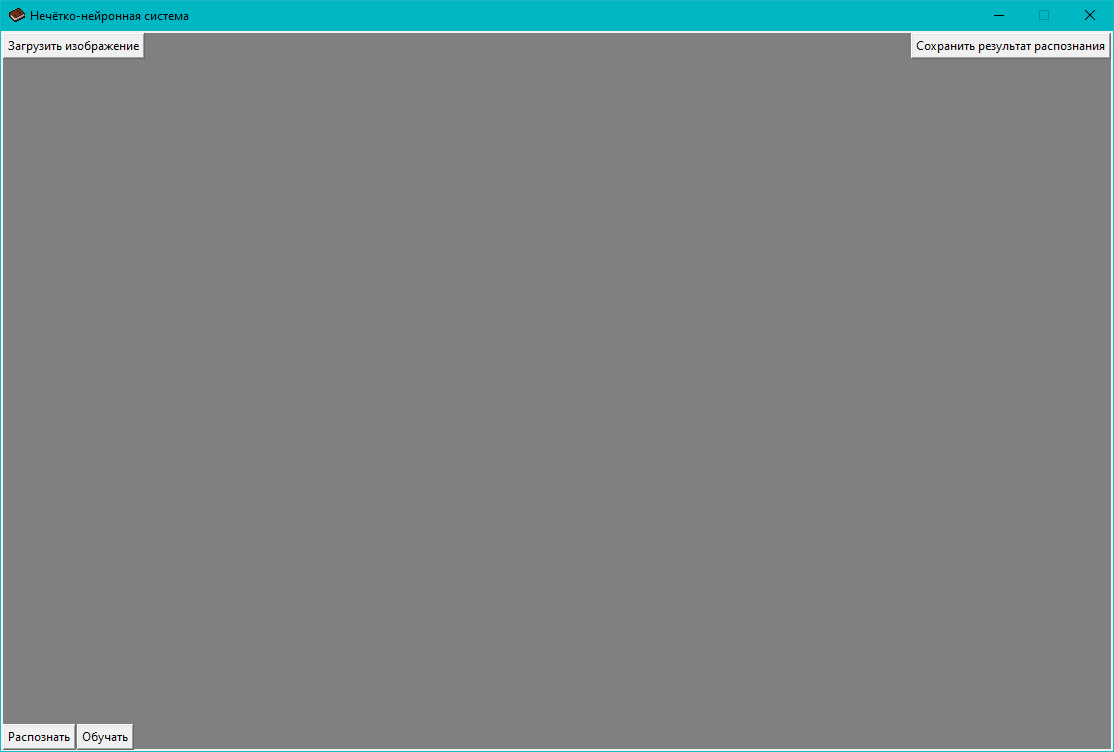
\includegraphics[width=1\linewidth]{systemtest_interface}
\caption{Диаграмма вариантов использования}
\label{systemtest_interface:image}
\end{figure}

На рисунках \ref{systemtest_responce:image}-\ref{systemtest_responce4:image} представлен полный путь распознания объекта на изображении.

\begin{figure}[H]
\center{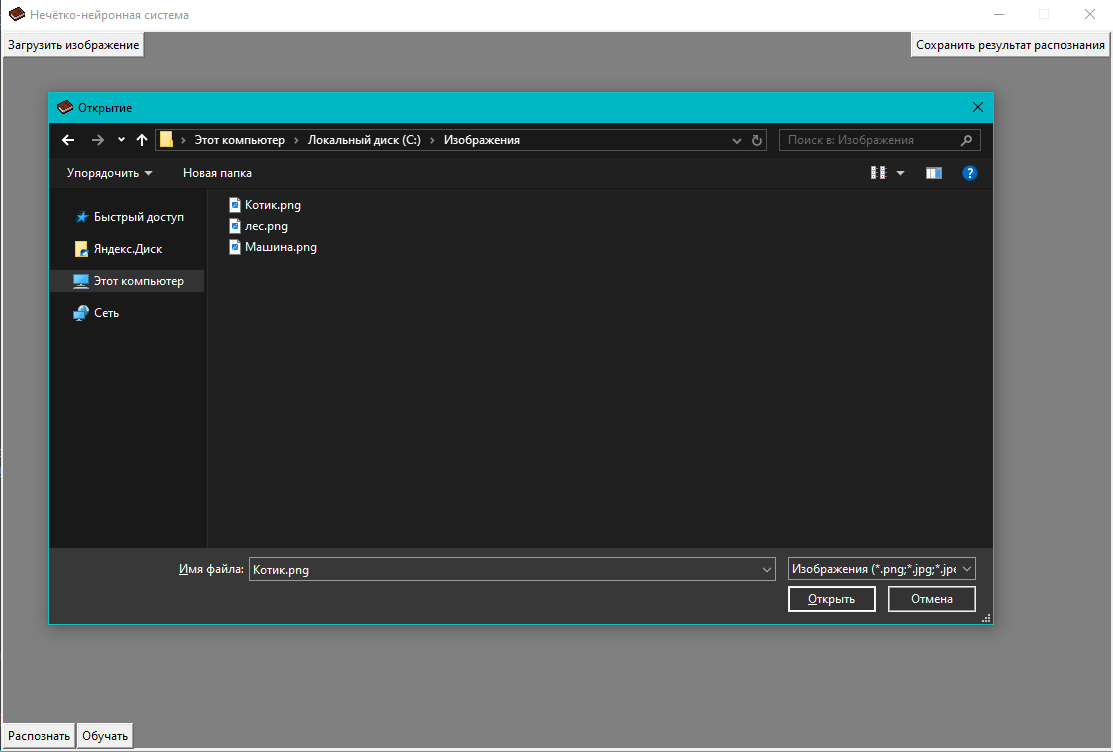
\includegraphics[width=1\linewidth]{systemtest_responce}}
\caption{Диалоговое окно загрузки файла Машина.png}
\label{systemtest_responce:image}
\end{figure}

\begin{figure}[H]
\center{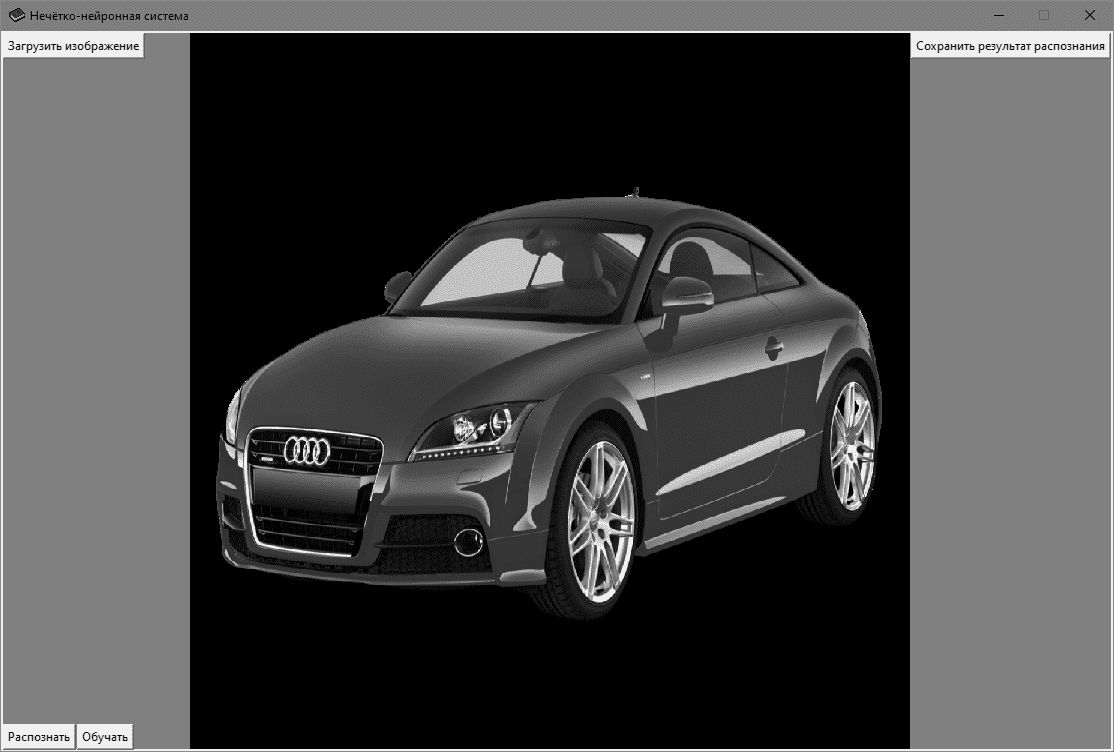
\includegraphics[width=1\linewidth]{systemtest_responce1}}
\caption{Изображение отображено в интерфейсе программы}
\label{systemtest_responce1:image}
\end{figure}

\begin{figure}[H]
\center{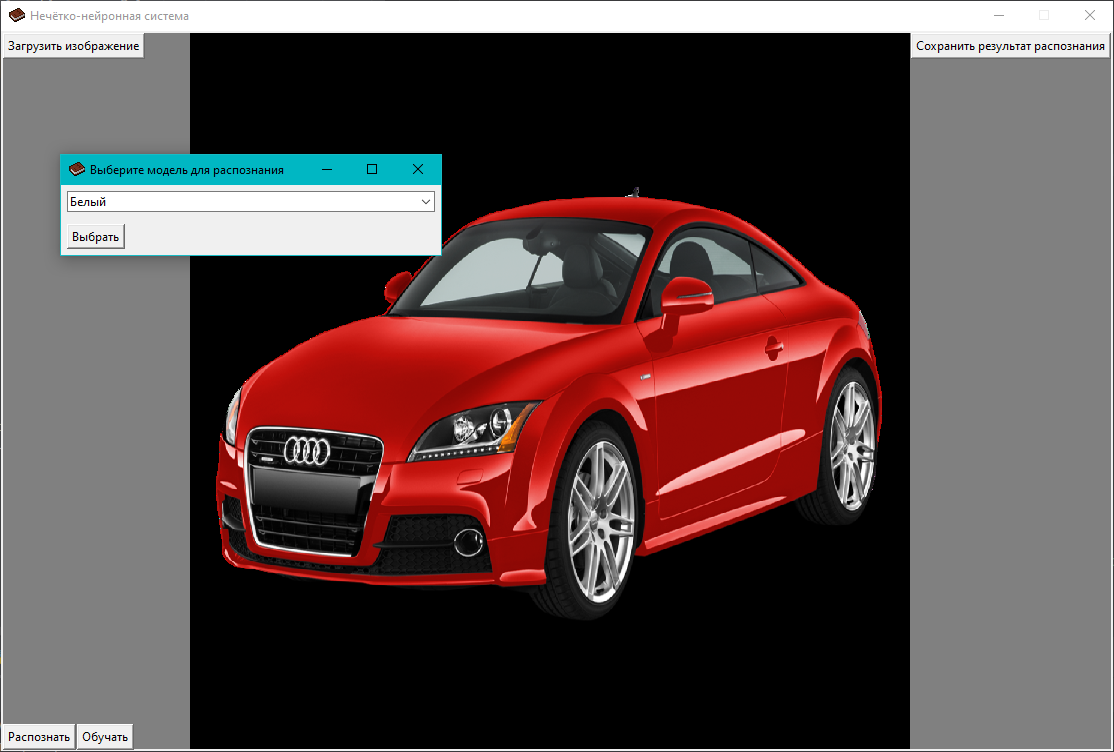
\includegraphics[width=1\linewidth]{systemtest_responce2}}
\caption{Окно выбора модели для распознания}
\label{systemtest_responce2:image}
\end{figure}

\begin{figure}[H]
\center{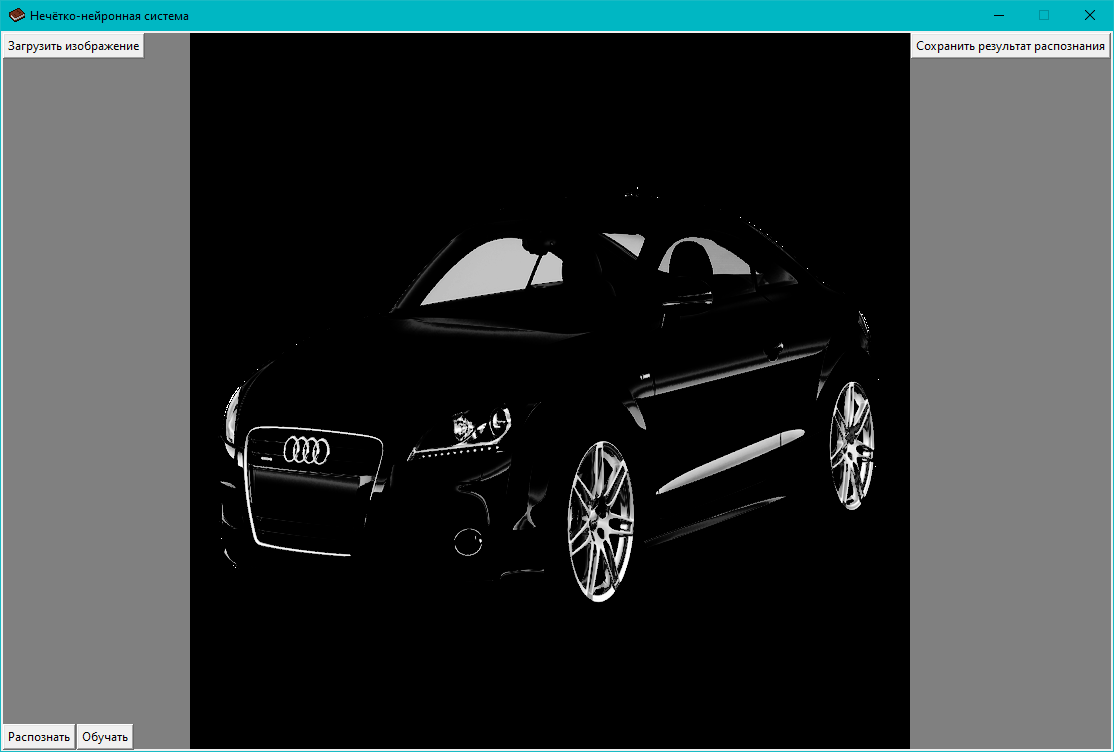
\includegraphics[width=1\linewidth]{systemtest_responce3}}
\caption{Распознанный объект отображен на интерфейсе}
\label{systemtest_responce3:image}
\end{figure}

\begin{figure}[H]
\center{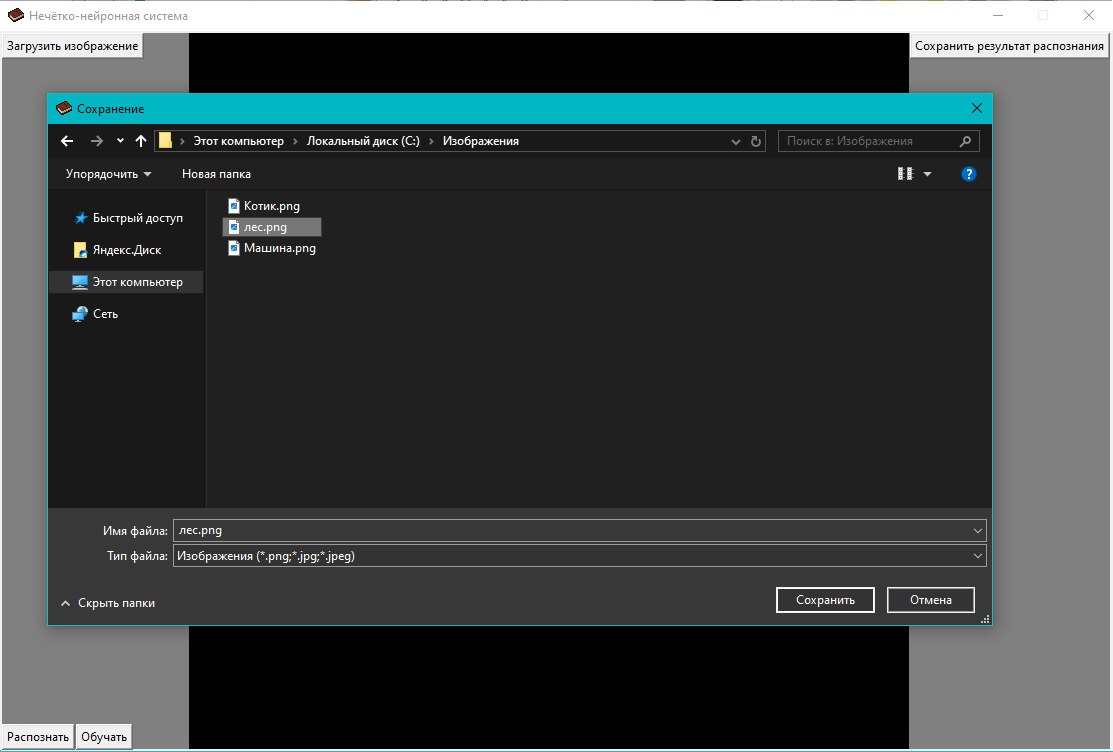
\includegraphics[width=1\linewidth]{systemtest_responce4}}
\caption{Диалоговое окно сохранения результата}
\label{systemtest_responce4:image}
\end{figure}

На рисунках \ref{systemtest_train1:image}-\ref{systemtest_train3:image} представлены все варианты обучения нейронной сети.

На рисунке \ref{systemtest_train1:image} была нажата кнопка обучать, после чего открылось окно выбора набора.

\begin{figure}[H]
\center{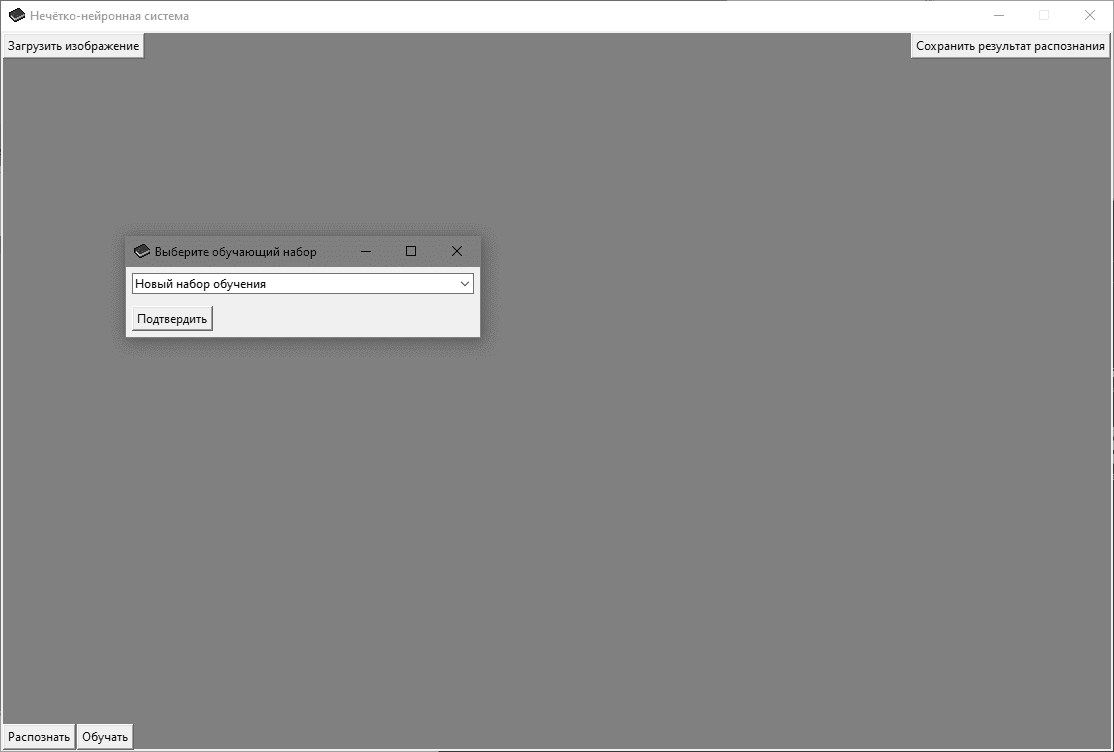
\includegraphics[width=1\linewidth]{systemtest_train1}}
\caption{Окно выбора обучающего набора}
\label{systemtest_train1:image}
\end{figure}

После выбора нового набора появилось окно, предлагающее назвать модель и обучить её.

\begin{figure}[H]
\center{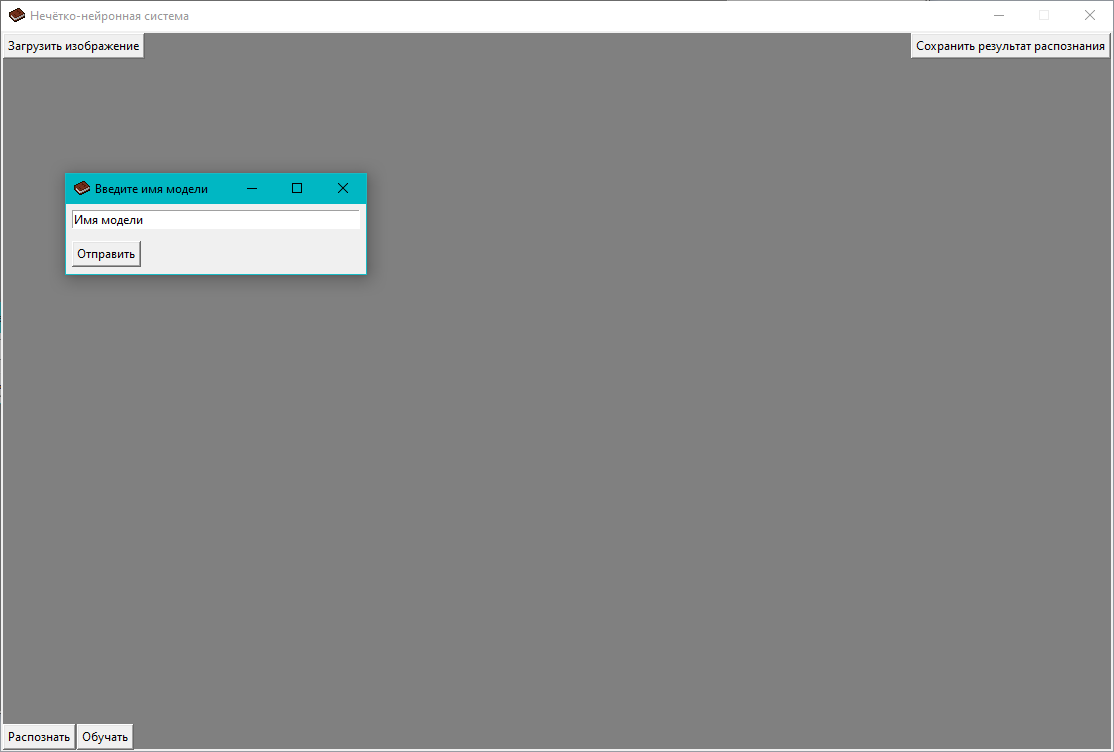
\includegraphics[width=1\linewidth]{systemtest_train2}}
\caption{Окно выбора названия новой модели}
\label{systemtest_train2:image}
\end{figure}

Вместо создания нового набора, после нажатия кнопки обучать, можно выбрать заготовленный набор и обучить нейронную сеть по нему.

\begin{figure}[H]
\center{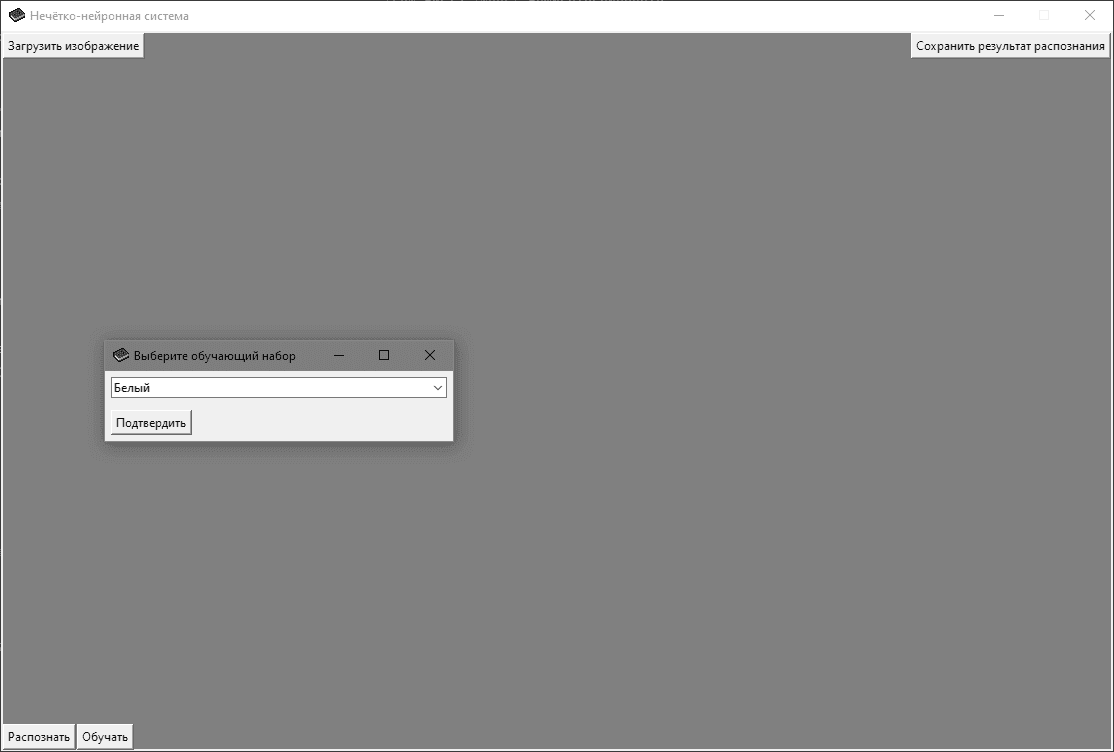
\includegraphics[width=1\linewidth]{systemtest_train3}}
\caption{Выбор обучения по набору ''Белый''}
\label{systemtest_train3:image}
\end{figure}

На рисунке \ref{systemtest_responce5:image} было загружено изображение кошки.

\begin{figure}[H]
\center{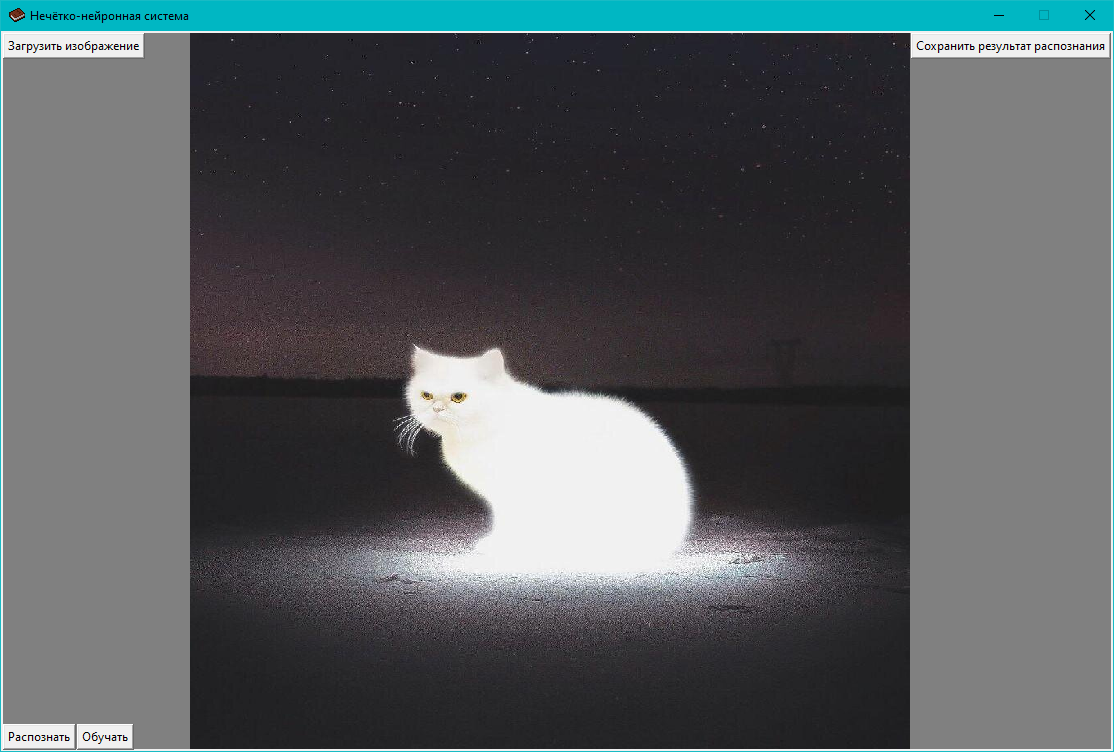
\includegraphics[width=1\linewidth]{systemtest_responce5}}
\caption{Интерфейс с изображением кошки}
\label{systemtest_responce5:image}
\end{figure}

На рисунке \ref{systemtest_responce6:image} изображение кошки было обработано по модели ''Белый''.

\begin{figure}[H]
\center{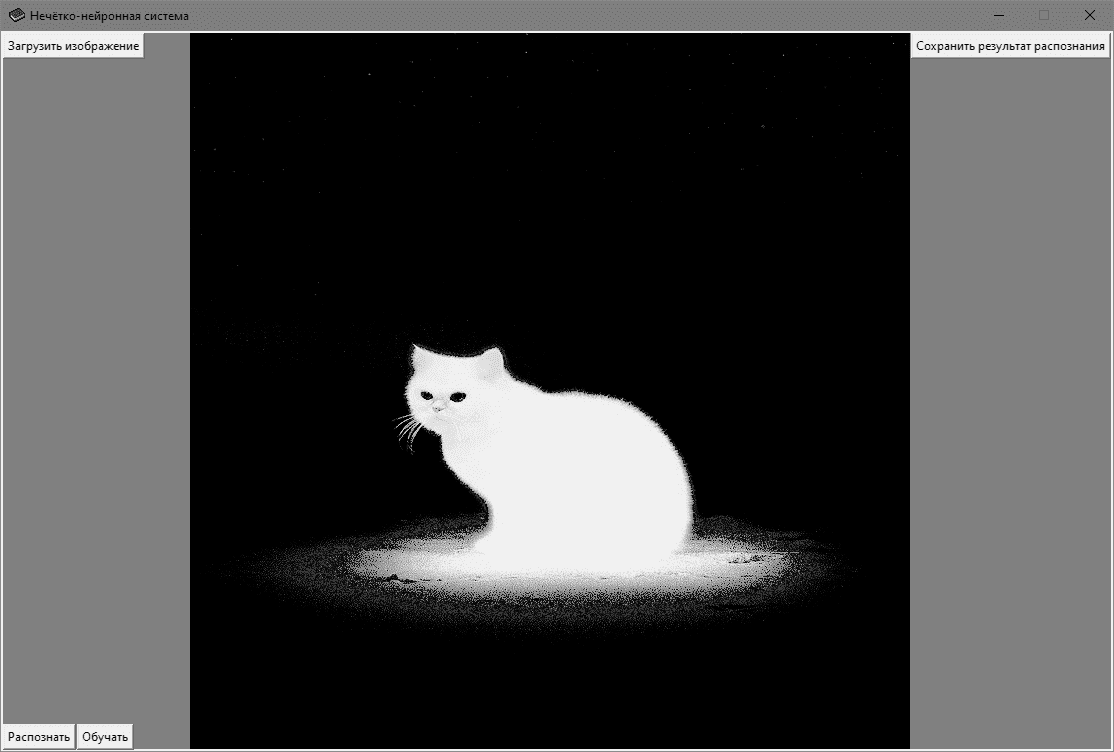
\includegraphics[width=1\linewidth]{systemtest_responce6}}
\caption{Распознанныйе объекты на изображении кошки}
\label{systemtest_responce6:image}
\end{figure}
На рисунке \ref{systemtest_responce7:image} было загружено изображение лилии.

\begin{figure}[H]
\center{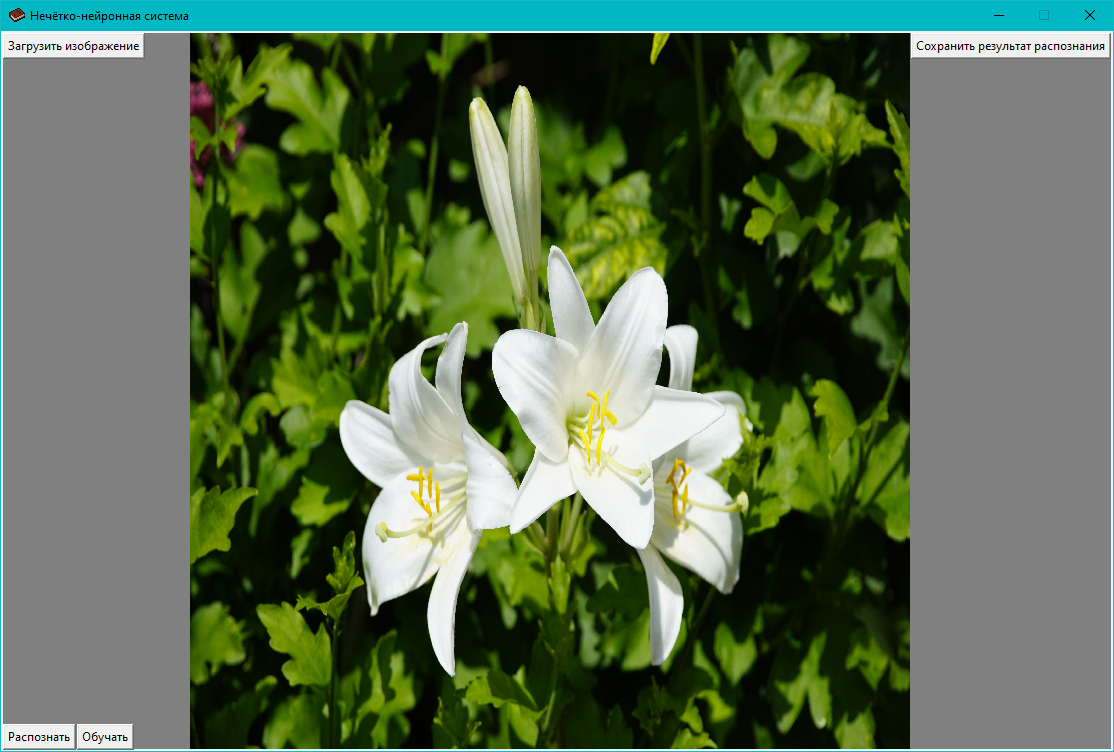
\includegraphics[width=1\linewidth]{systemtest_responce7}}
\caption{Интерфейс с изображением лилии}
\label{systemtest_responce7:image}
\end{figure}

На рисунке \ref{systemtest_responce8:image} изображение лилии было обработано по модели ''Белый''.

\begin{figure}[H]
\center{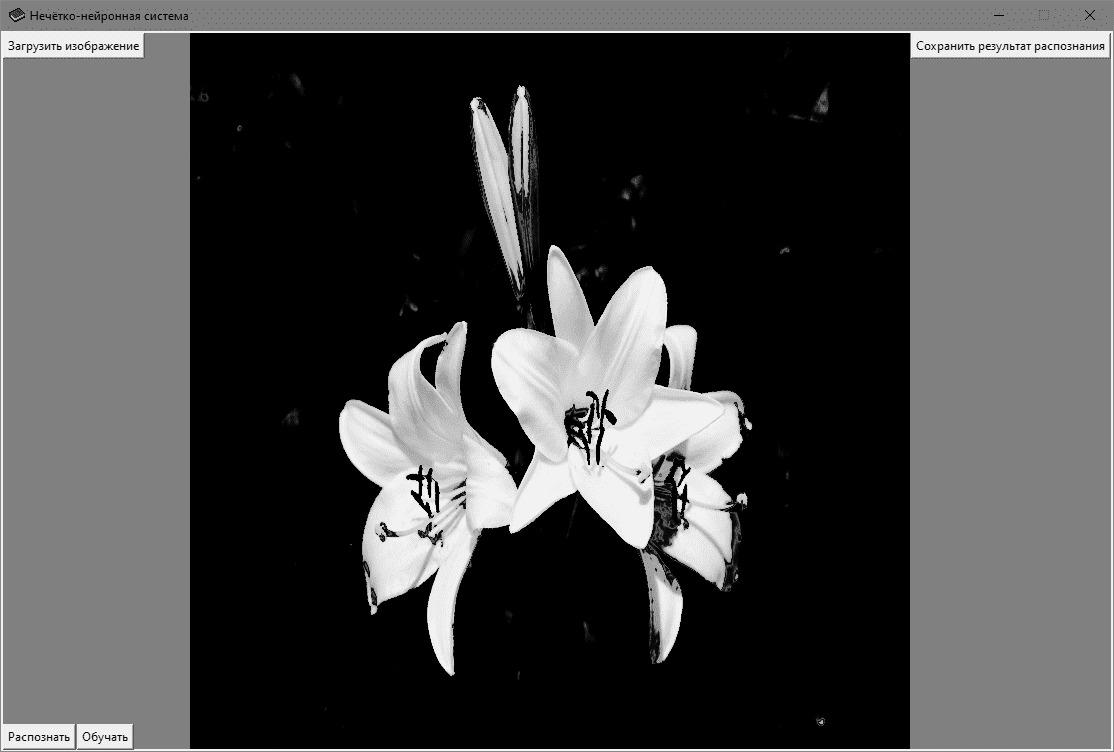
\includegraphics[width=1\linewidth]{systemtest_responce8}}
\caption{Распознанныйе объекты на изображении лилии}
\label{systemtest_responce8:image}
\end{figure}
На рисунке \ref{systemtest_responce9:image} было загружено изображение леса.

\begin{figure}[H]
\center{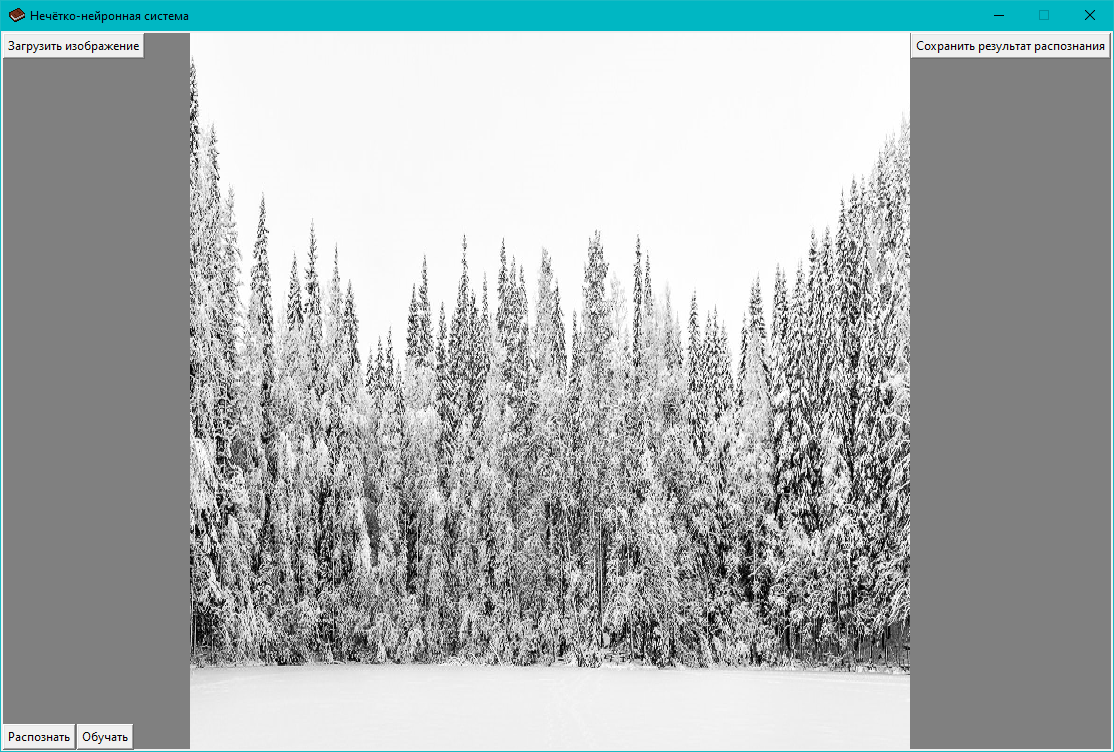
\includegraphics[width=1\linewidth]{systemtest_responce9}}
\caption{Интерфейс с изображением леса}
\label{systemtest_responce9:image}
\end{figure}

На рисунке \ref{systemtest_responce10:image} изображение леса было обработано по модели ''Белый''.

\begin{figure}[H]
\center{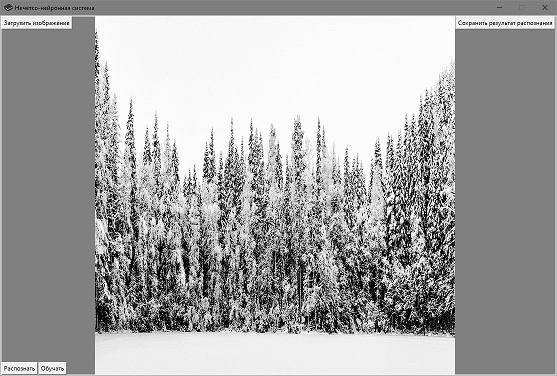
\includegraphics[width=1\linewidth]{systemtest_responce10}}
\caption{Распознанныйе объекты на изображении леса}
\label{systemtest_responce10:image}
\end{figure}
На рисунке \ref{systemtest_responce11:image} было загружено изображение футбола.

\begin{figure}[H]
\center{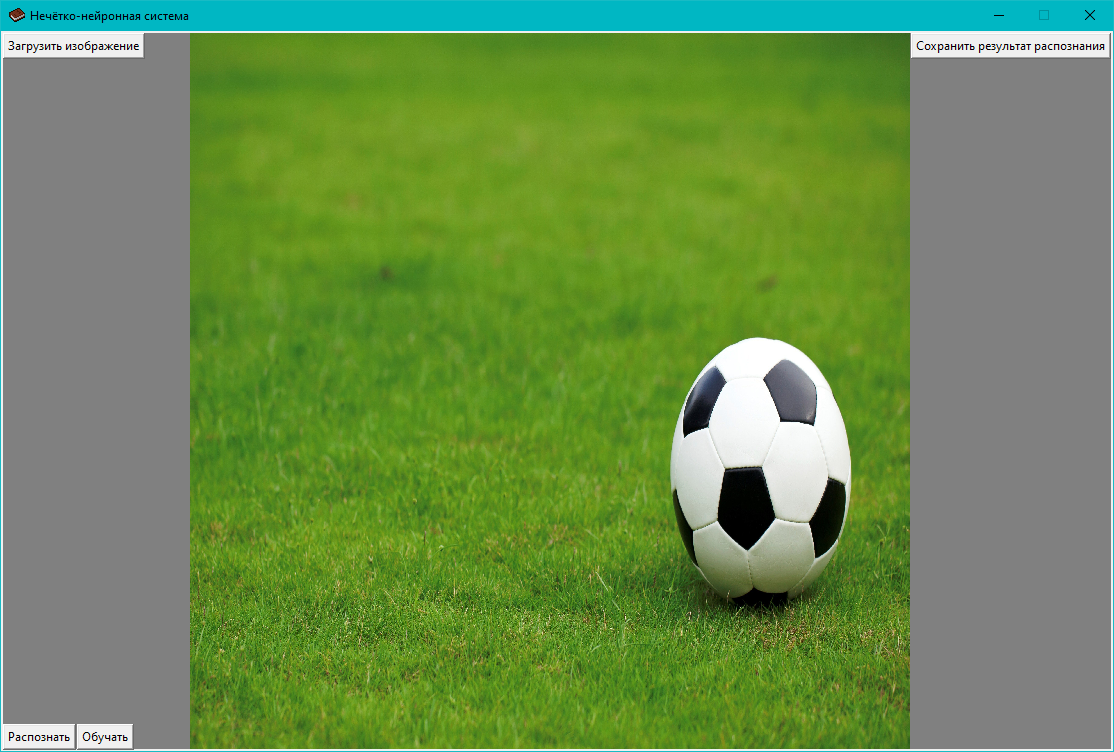
\includegraphics[width=1\linewidth]{systemtest_responce11}}
\caption{Интерфейс с изображением футбола}
\label{systemtest_responce11:image}
\end{figure}

На рисунке \ref{systemtest_responce12:image} изображение футбола было обработано по модели ''Белый''.

\begin{figure}[H]
\center{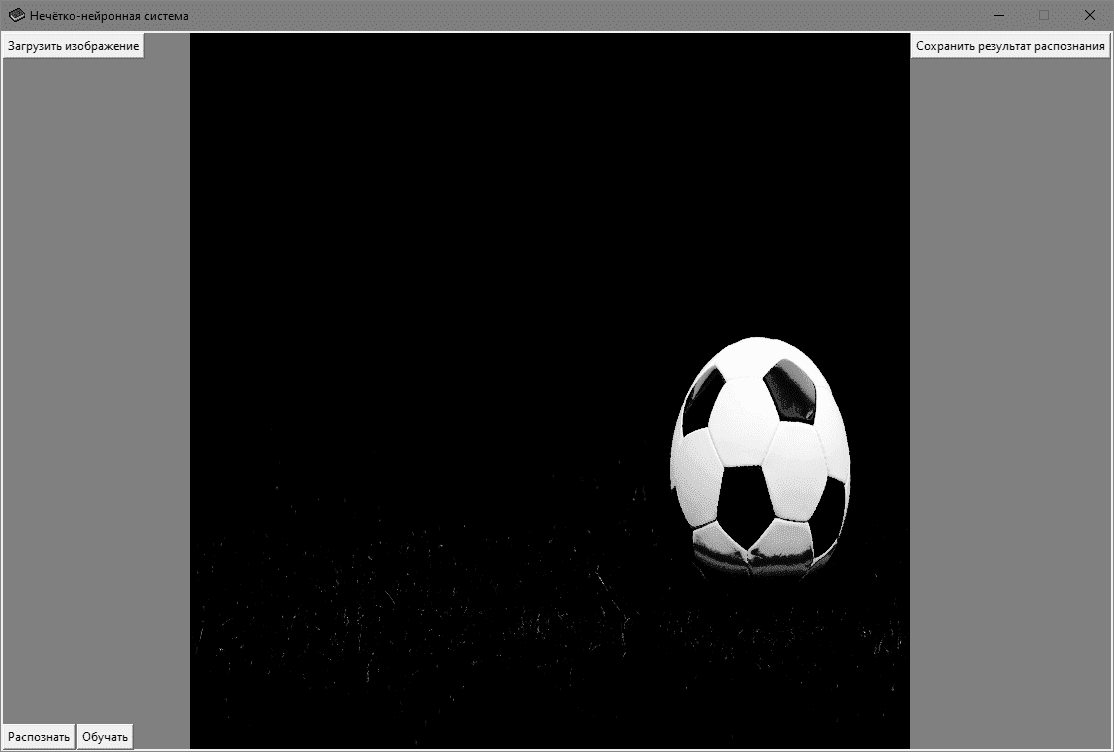
\includegraphics[width=1\linewidth]{systemtest_responce12}}
\caption{Распознанныйе объекты на изображении футбола}
\label{systemtest_responce12:image}
\end{figure}
На рисунке \ref{systemtest_responce13:image} было загружено изображение платья.

\begin{figure}[H]
\center{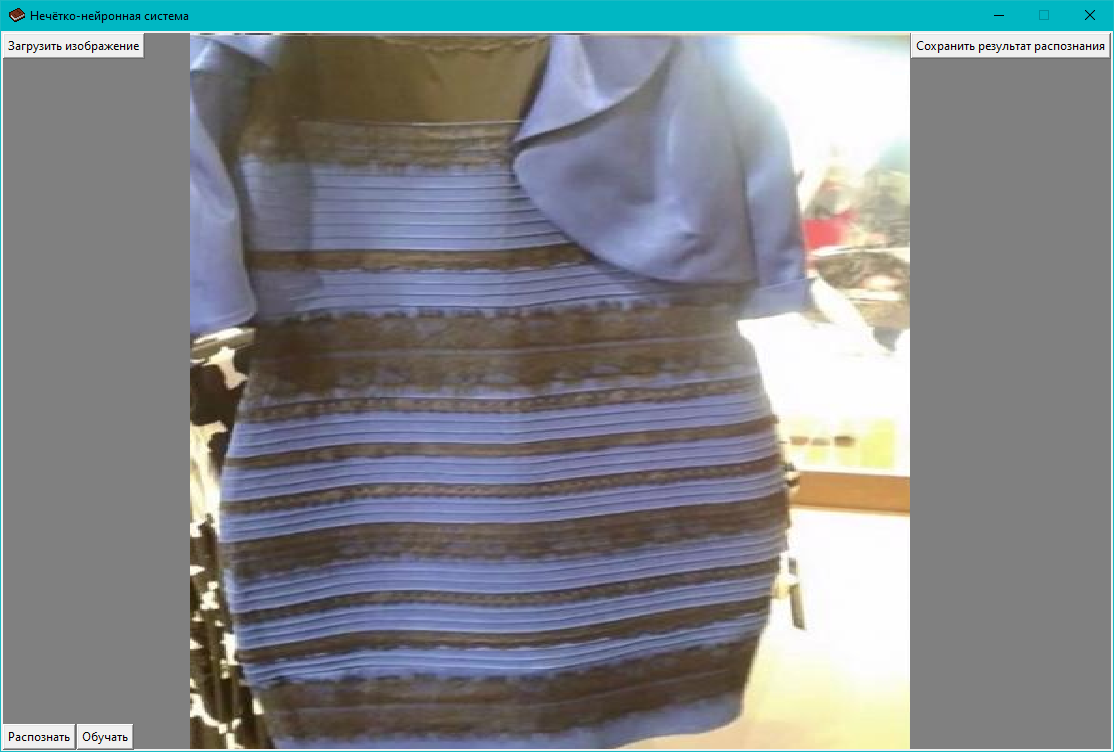
\includegraphics[width=1\linewidth]{systemtest_responce13}}
\caption{Интерфейс с изображением платья}
\label{systemtest_responce13:image}
\end{figure}

На рисунке \ref{systemtest_responce14:image} изображение платья было обработано по модели ''Белый''.

\begin{figure}[H]
\center{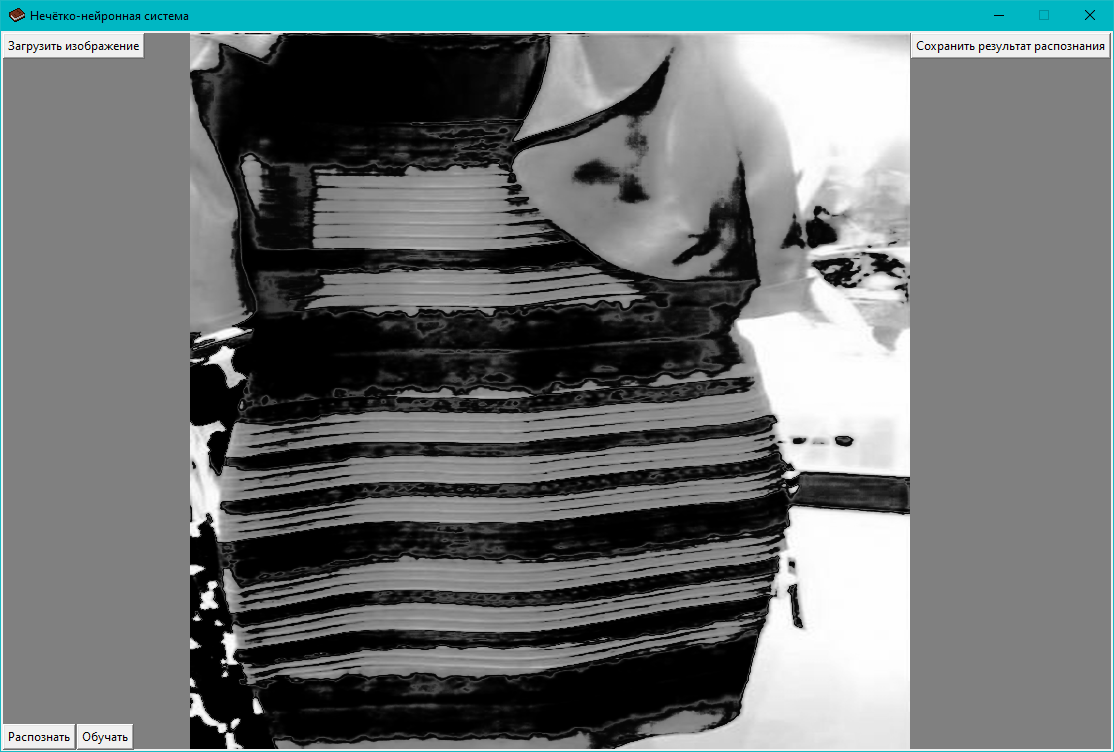
\includegraphics[width=1\linewidth]{systemtest_responce14}}
\caption{Распознанныйе объекты на изображении платья}
\label{systemtest_responce14:image}
\end{figure}

На рисунке \ref{systemtest_responce15:image} было загружено изображение берёзы.

\begin{figure}[H]
\center{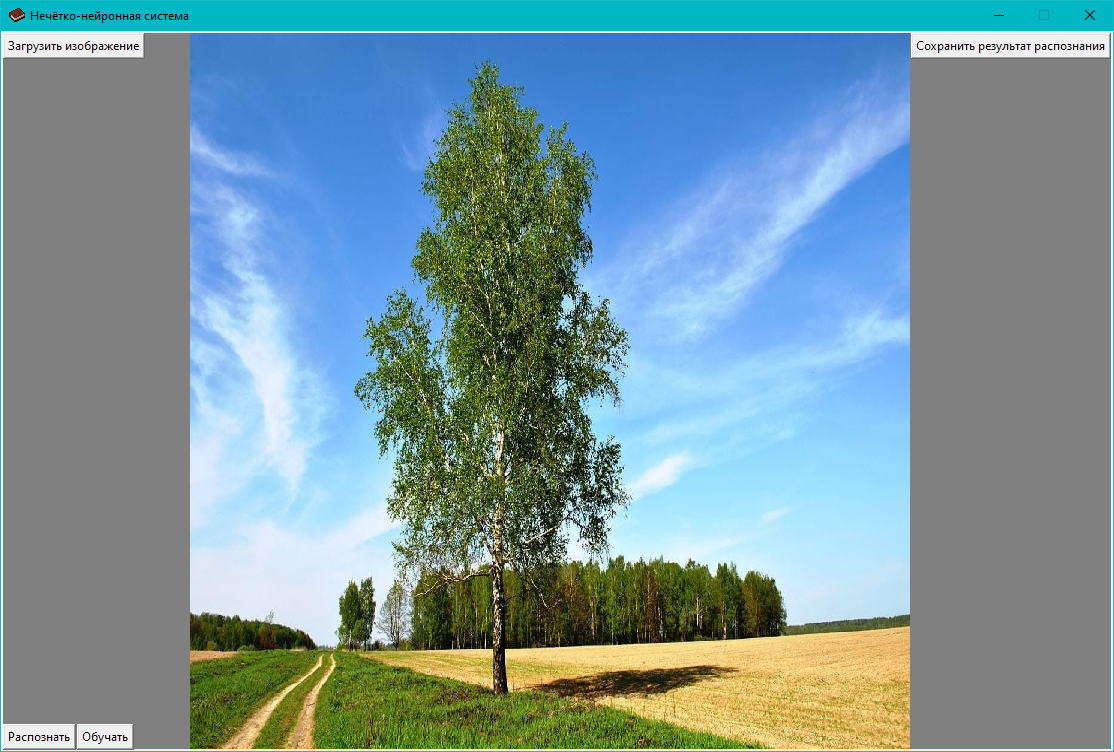
\includegraphics[width=1\linewidth]{systemtest_responce15}}
\caption{Интерфейс с изображением берёзы}
\label{systemtest_responce15:image}
\end{figure}

На рисунке \ref{systemtest_responce16:image} изображение берёзы было обработано по модели ''Белый''.

\begin{figure}[H]
\center{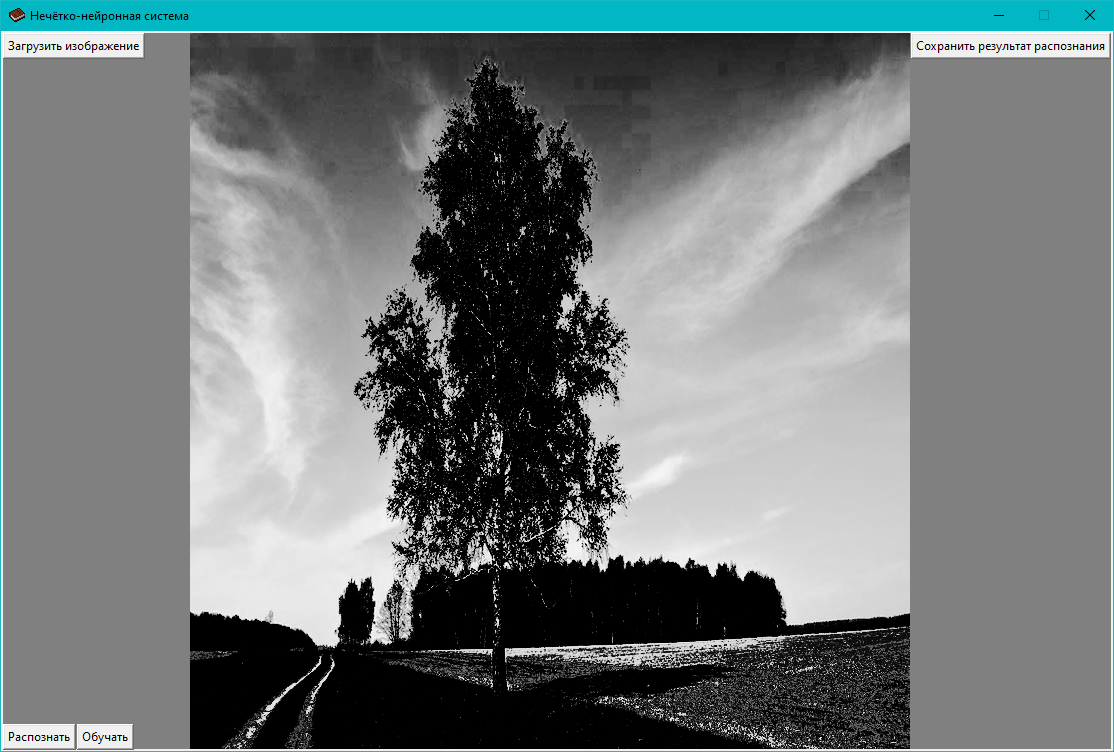
\includegraphics[width=1\linewidth]{systemtest_responce16}}
\caption{Распознанныйе объекты на изображении берёзы}
\label{systemtest_responce16:image}
\end{figure}

На рисунке \ref{systemtest_responce17:image} было загружено изображение дварфа.

\begin{figure}[H]
\center{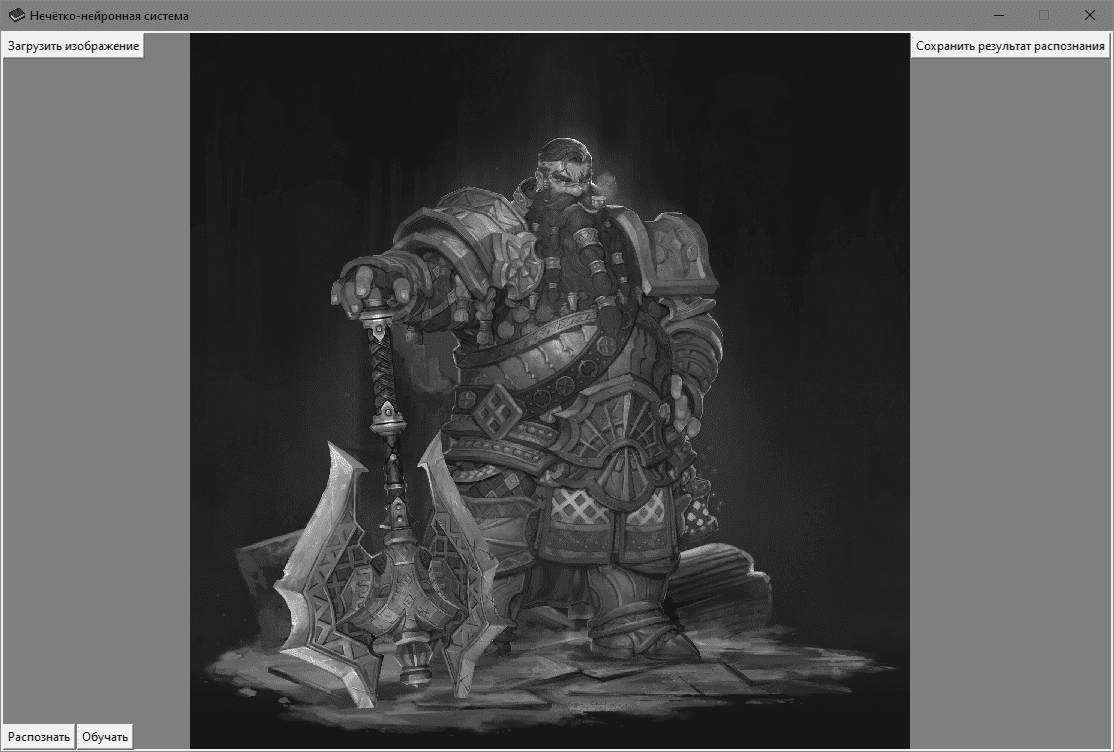
\includegraphics[width=1\linewidth]{systemtest_responce17}}
\caption{Интерфейс с изображением дварфа}
\label{systemtest_responce17:image}
\end{figure}

На рисунке \ref{systemtest_responce18:image} изображение дварфа было обработано по модели ''Белый''.

\begin{figure}[H]
\center{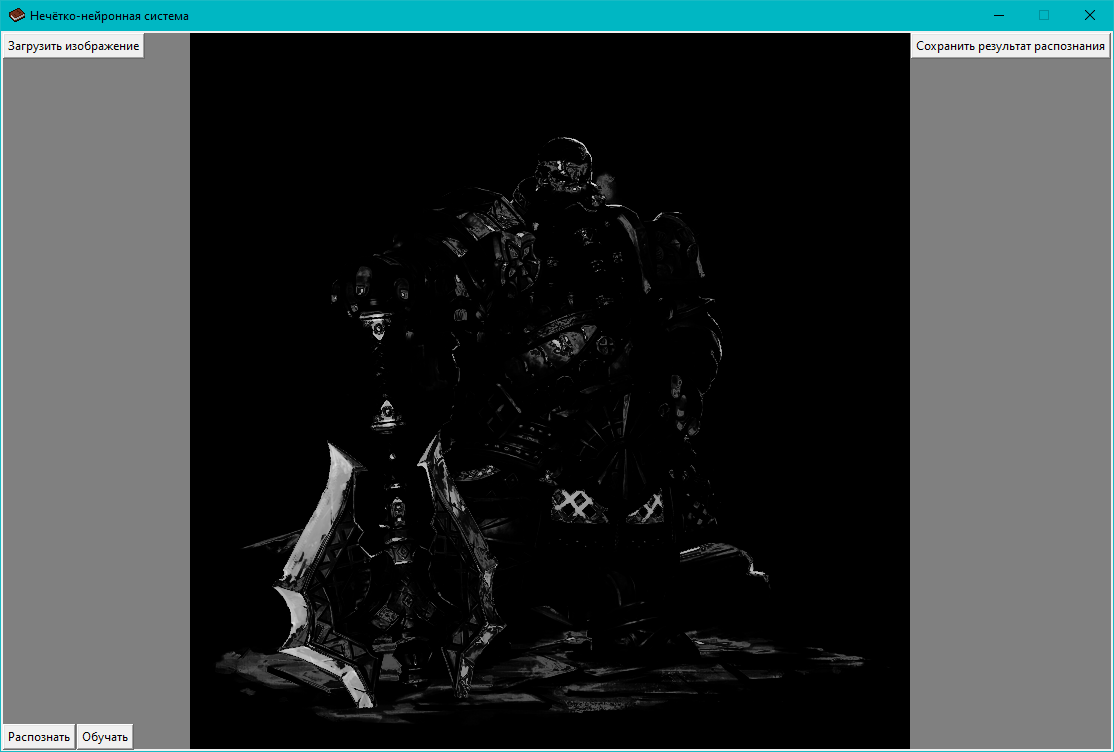
\includegraphics[width=1\linewidth]{systemtest_responce18}}
\caption{Распознанныйе объекты на изображении дварфа}
\label{systemtest_responce18:image}
\end{figure}
На рисунке \ref{systemtest_responce19:image} было загружено изображение Чебурашки.

\begin{figure}[H]
\center{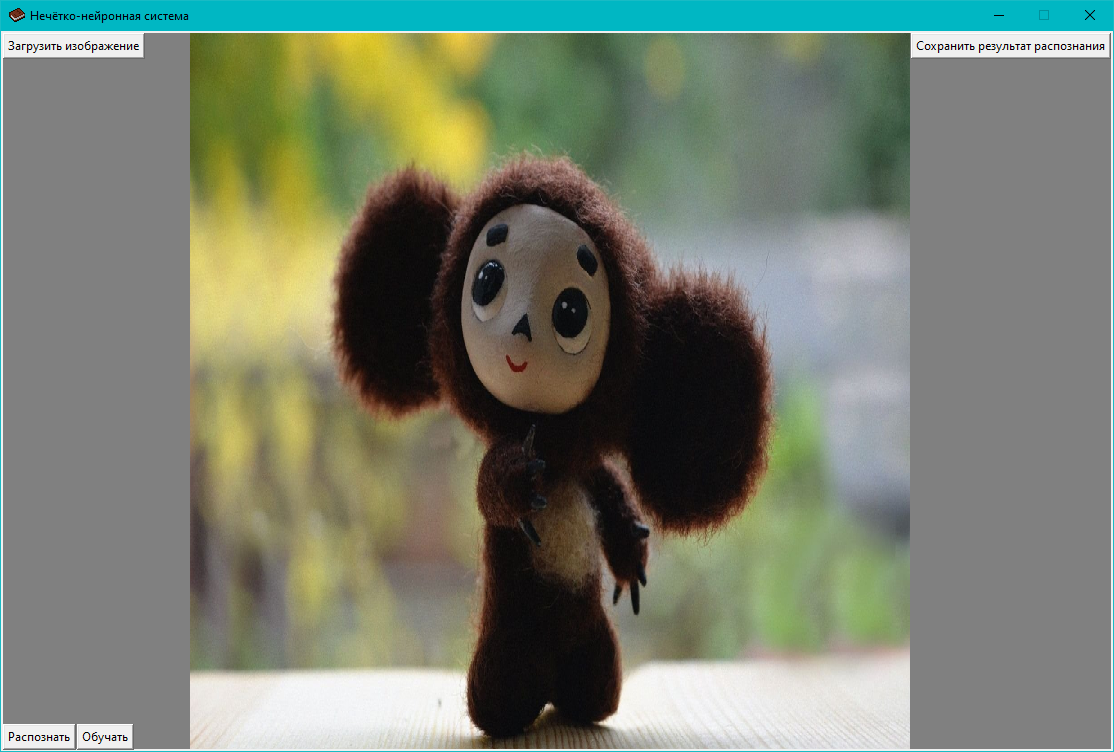
\includegraphics[width=1\linewidth]{systemtest_responce19}}
\caption{Интерфейс с изображением Чебурашки}
\label{systemtest_responce19:image}
\end{figure}

На рисунке \ref{systemtest_responce20:image} изображение Чебурашки было обработано по модели ''Белый''.

\begin{figure}[H]
\center{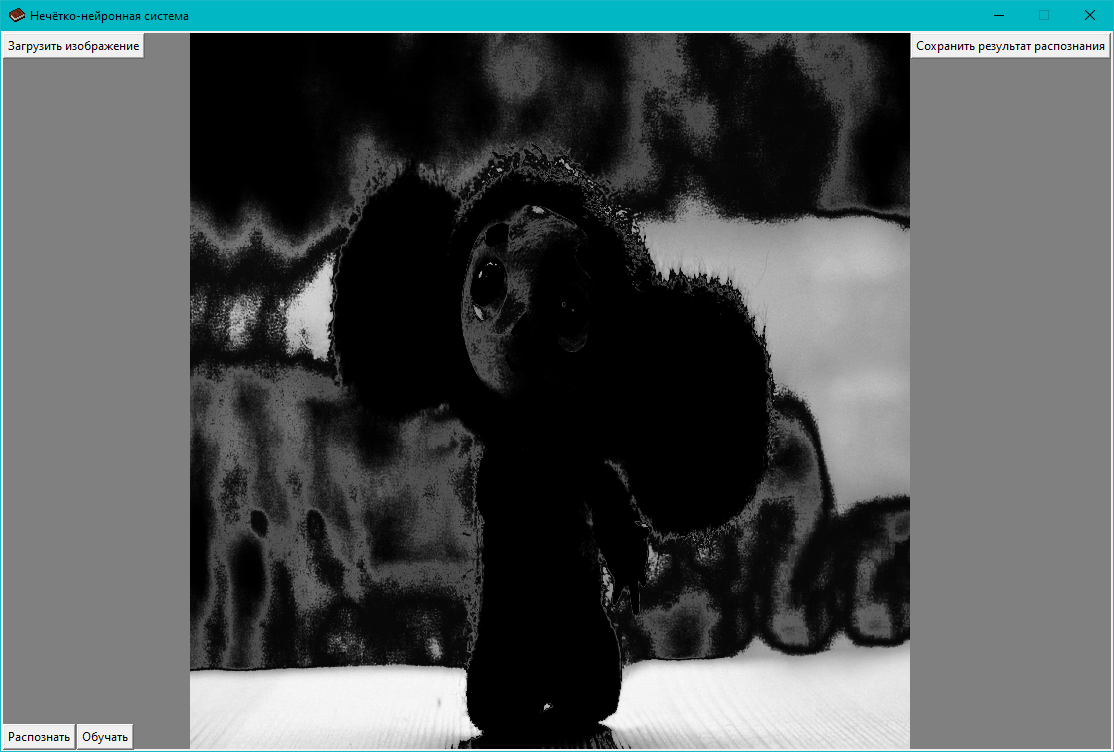
\includegraphics[width=1\linewidth]{systemtest_responce20}}
\caption{Распознанныйе объекты на изображении Чебурашки}
\label{systemtest_responce20:image}
\end{figure}

На рисунке \ref{systemtest_responce21:image} было загружено изображение поезда.

\begin{figure}[H]
\center{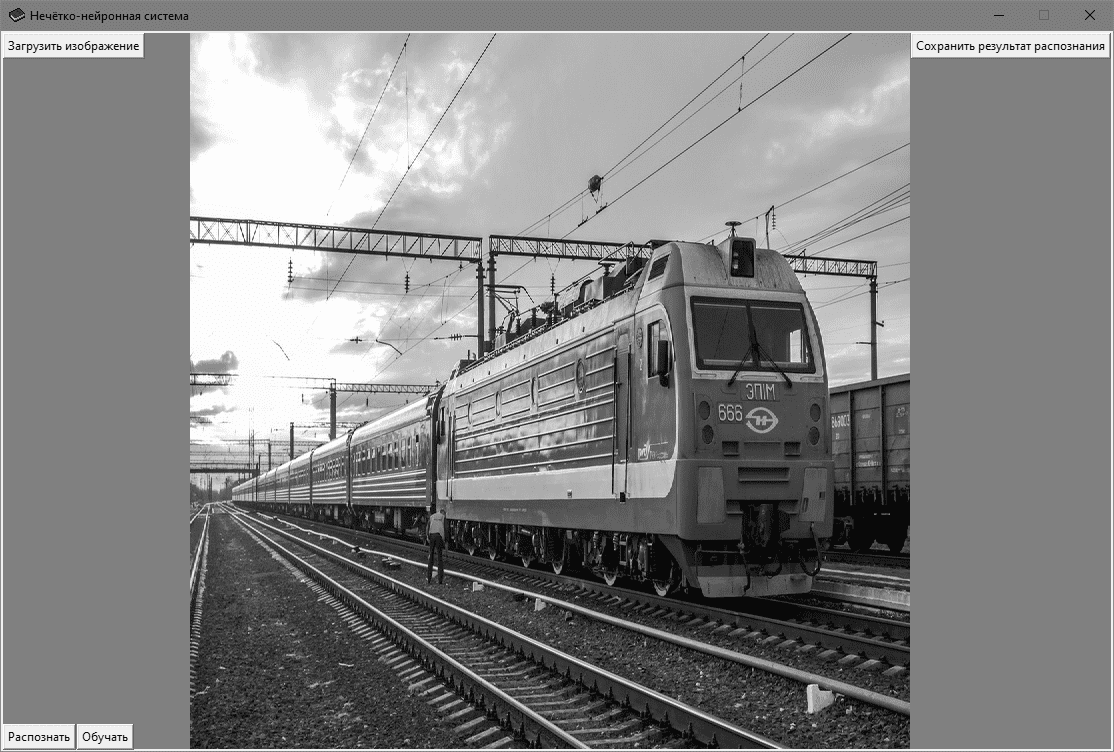
\includegraphics[width=1\linewidth]{systemtest_responce21}}
\caption{Интерфейс с изображением поезда}
\label{systemtest_responce21:image}
\end{figure}

На рисунке \ref{systemtest_responce22:image} изображение поезда было обработано по модели ''Белый''.

\begin{figure}[H]
\center{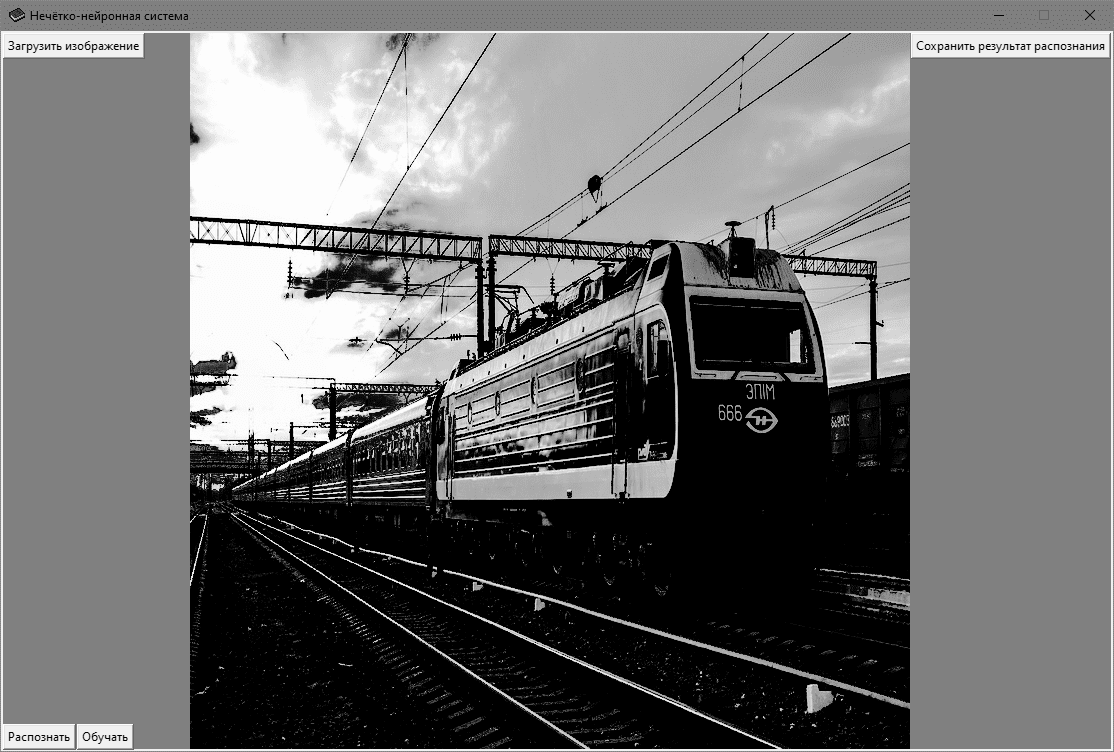
\includegraphics[width=1\linewidth]{systemtest_responce22}}
\caption{Распознанныйе объекты на изображении поезда}
\label{systemtest_responce22:image}
\end{figure}

На рисунке \ref{systemtest_responce23:image} было загружено изображение мафинов.

\begin{figure}[H]
\center{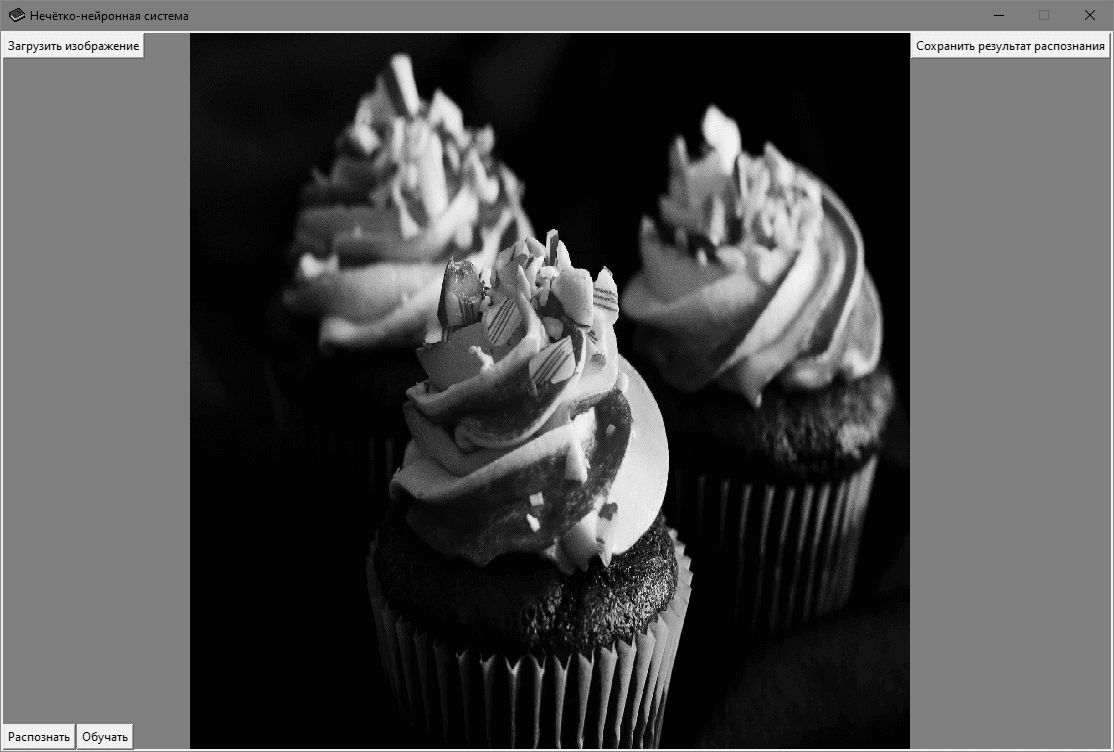
\includegraphics[width=1\linewidth]{systemtest_responce23}}
\caption{Интерфейс с изображением мафинов}
\label{systemtest_responce23:image}
\end{figure}

На рисунке \ref{systemtest_responce24:image} изображение мафинов было обработано по модели ''Белый''.

\begin{figure}[H]
\center{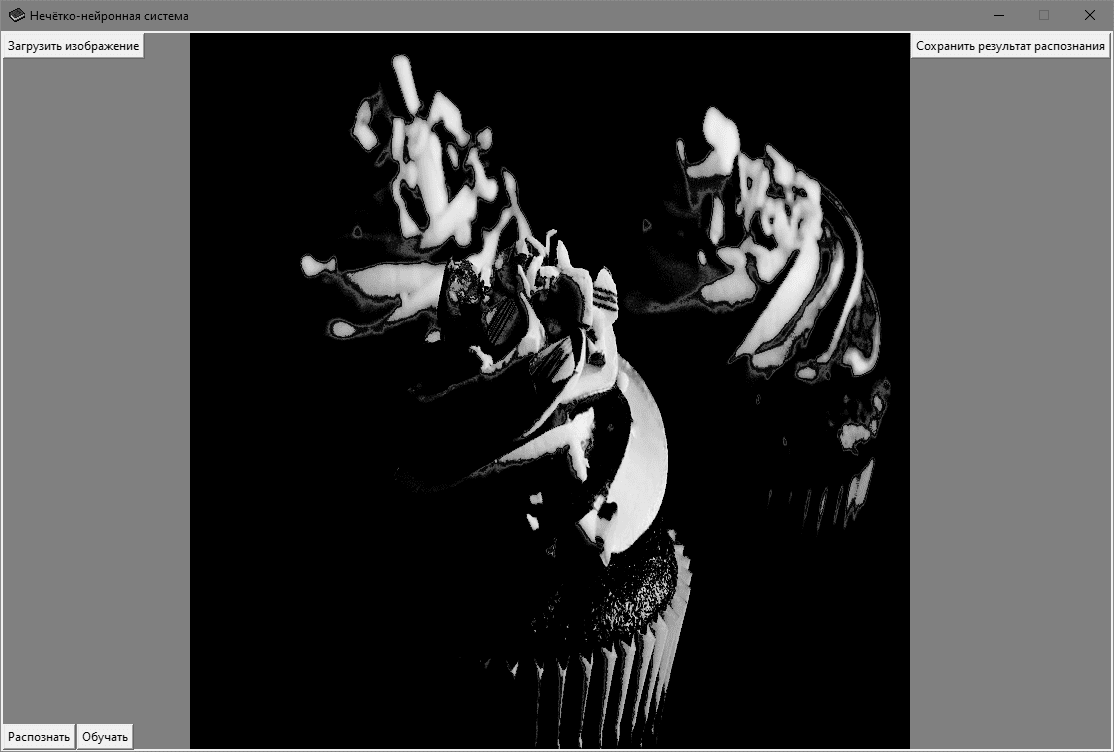
\includegraphics[width=1\linewidth]{systemtest_responce24}}
\caption{Распознанныйе объекты на изображении мафинов}
\label{systemtest_responce24:image}
\end{figure}